\documentclass[aspectratio=169,10pt]{beamer}

\usetheme[progressbar=frametitle,noslidenumbers]{metropolis}
\usepackage{appendixnumberbeamer}

\usepackage{booktabs}
\usepackage[scale=2]{ccicons}

\usepackage{tikz}
\usetikzlibrary{patterns,arrows,calc}

\usepackage{pgfplots}
\usepgfplotslibrary{dateplot,fillbetween}
\usepackage[super]{nth}
\usepackage{xspace}
\usepackage{url}
\newcommand{\themename}{\textbf{\textsc{metropolis}}\xspace}

% color palette
\definecolor{tu01}{HTML}{84B818}
\definecolor{tu02}{HTML}{D18B12}
\definecolor{tu03}{HTML}{1BB5B5}
\definecolor{tu04}{HTML}{F85A3E}
\definecolor{tu05}{HTML}{4B6CFC}
\definecolor{tu06}{HTML}{E3B505}
\definecolor{tu07}{HTML}{AF331D}
\definecolor{tu08}{HTML}{000000}
\definecolor{tu09}{HTML}{AAAAAA}
\definecolor{tu10}{HTML}{444444}
\definecolor{tu11}{HTML}{84B818}

% mixed and light colors
\colorlet{tu01light}{tu01!33}
\colorlet{tu02light}{tu02!33}
\colorlet{tu03light}{tu03!33}
\colorlet{tu04light}{tu04!33}
\colorlet{tu05light}{tu05!33}
\colorlet{tu06light}{tu06!33}
\colorlet{tu07light}{tu07!33}
\colorlet{tu08light}{tu08!33}
\colorlet{tu09light}{tu09!33}
\colorlet{tu10light}{tu10!33}
\colorlet{tu11light}{tu11!33}

\colorlet{tu01midlight}{tu01!50}
\colorlet{tu02midlight}{tu02!50}
\colorlet{tu03midlight}{tu03!50}
\colorlet{tu04midlight}{tu04!50}
\colorlet{tu05midlight}{tu05!50}
\colorlet{tu06midlight}{tu06!50}
\colorlet{tu07midlight}{tu07!50}
\colorlet{tu08midlight}{tu08!50}
\colorlet{tu09midlight}{tu09!50}
\colorlet{tu10midlight}{tu10!50}
\colorlet{tu11midlight}{tu11!50}

\colorlet{tu01dark}{tu01!80!black}
\colorlet{tu02dark}{tu02!80!black}
\colorlet{tu03dark}{tu03!80!black}
\colorlet{tu04dark}{tu04!80!black}
\colorlet{tu05dark}{tu05!80!black}
\colorlet{tu06dark}{tu06!80!black}
\colorlet{tu07dark}{tu07!80!black}
\colorlet{tu08dark}{tu08!80!black}
\colorlet{tu09dark}{tu09!80!black}
\colorlet{tu10dark}{tu10!80!black}
\colorlet{tu11dark}{tu11!80!black}

\colorlet{lightgray}{gray!25}
\colorlet{midlightgray}{gray!50}
\colorlet{anthracite}{black!85}

% aliases
\colorlet{tudo}{tu01}
\colorlet{tuorange}{tu02}
\colorlet{tudolight}{tu01light}
% 'axis line on top' option
\makeatletter \newcommand{\pgfplotsdrawaxis}{\pgfplots@draw@axis} \makeatother
\pgfplotsset{axis line on top/.style={
  axis line style = transparent,
  ticklabel style = transparent,
  tick style = transparent,
  axis on top = false,
  after end axis/.append code = {
    \pgfplotsset{
      axis line style = opaque,
      ticklabel style = opaque,
      tick style = opaque,
      grid = none
    }
    \pgfplotsdrawaxis
  }
}}

% enables animations in plots
\tikzset{
  invisible/.style={%
    opacity=0,
    mark options = {opacity=0},
    every error bar/.append style = {opacity=0}
  },
  visible on/.style={alt={#1{}{invisible}}},
  alt/.code args={<#1>#2#3}{%
    \alt<#1>{\pgfkeysalso{#2}}{\pgfkeysalso{#3}} % \pgfkeysalso doesn't change the path
  },
}

% elegant legend on the outside
\pgfplotsset{outside legend/.style = {
  legend style = {
    draw = none,
    fill = none,
    at = {(1.025,.5)},
    anchor = west,
    row sep = .25em
  }
}}

% default axis style
\pgfplotsset{default axis/.style = {
  axis line on top,
  axis line style = {anthracite, semithick},
  axis background/.style = {fill = white},
  legend cell align = {left},
  scaled y ticks = false
}}

% histograms
\pgfplotsset{histogram axis/.style = {
  default axis,
  legend style = {
    at = {(0.98,0.02)},
    anchor = south east
  },
  legend cell align = left
}}

\pgfplotsset{histogram plot/.style = {
  const plot,
  mark = none
}}

% progress plots
\pgfplotsset{progress axis/.style = {
  default axis
}}

\pgfplotsset{progress plot/.style = {
  semithick,
  solid
}}

% marks for progress plots
\pgfplotsset{m00/.style = {mark = none, opacity = 1, anthracite, densely dashed}}
\pgfplotsset{m01/.style = {tu01!33, mark options = {draw=tu01, scale = 1.2, fill=white}, every error bar/.style = {tu01!66}, mark = *}}
\pgfplotsset{m02/.style = {tu02!33, mark options = {draw=tu02, scale = 1.2, fill=white}, every error bar/.style = {tu02!66}, mark = square*}}
\pgfplotsset{m03/.style = {tu03!33, mark options = {draw=tu03, scale = 1.2, fill=white}, every error bar/.style = {tu03!66}, mark = triangle*}}
\pgfplotsset{m04/.style = {tu04!33, mark options = {draw=tu04, scale = 1.2, fill=white}, every error bar/.style = {tu04!66}, mark = diamond*}}
\pgfplotsset{m05/.style = {tu05!33, mark options = {draw=tu05, scale = 1.2, fill=white}, every error bar/.style = {tu05!66}, mark = pentagon*}}
\pgfplotsset{m06/.style = {tu06!33, mark options = {draw=tu06, scale = 1.2, fill=white}, every error bar/.style = {tu06!66}, mark = otimes*}}
\pgfplotsset{m07/.style = {tu07!33, mark options = {draw=tu07, scale = 1.2, fill=white}, every error bar/.style = {tu07!66}, mark = oplus*}}
\pgfplotsset{m08/.style = {tu08!33, mark options = {draw=tu08, scale = 1.2, fill=white}, every error bar/.style = {tu08!66}, mark = star*}}
\pgfplotsset{m09/.style = {tu09!33, mark options = {draw=tu09, scale = 1.2, fill=white}, every error bar/.style = {tu09!66}, mark = x}}
\pgfplotsset{m10/.style = {tu10!33, mark options = {draw=tu10, scale = 1.2, fill=white}, every error bar/.style = {tu10!66}, mark = +}}
\pgfplotsset{m11/.style = {tu11!33, mark options = {draw=tu11, scale = 1.2, fill=white}, every error bar/.style = {tu11!66}, mark = |}}
% also: 'asterisk', '-', and most of the above without '*'


\title{Frameworks, Tools and Workflows}
\subtitle{and their impact on science}
% \date{\today}
\date{October \nth{25}, 2018}
\author{Lukas Pfahler}
\institute{TU Dortmund University, Chair for Artificial Intelligence}
\titlegraphic{\hfill
\includegraphics[height=8mm]{tu-do-logo.pdf}}

\begin{document}

\maketitle
\section{ReadMe}
\begin{frame}{Intention}
Goal of this DuD is to
\begin{itemize}
    \item present tools or frameworks you use frequently
    \item present how you use them: \textbf{Characteristic Workflows}
    \item discuss how they align with the principles of good research (correctness, reproducibility, documentation, collaboration, rapid-prototyping, ...)
\end{itemize}
The goal is \textbf{not} to
\begin{itemize}
    \item preach or proselytize
    \item bash other tools, workflows or ideas
    \item give a full tutorial
\end{itemize}
You get 2-3 slides to discuss your toolchain and what you like/dislike about it.
\end{frame}

% 1. Beitrag (Beispiel)
\section{Example Person}
% Let's start with an eye-catcher
\begin{frame}[fragile]{RapidMiner}
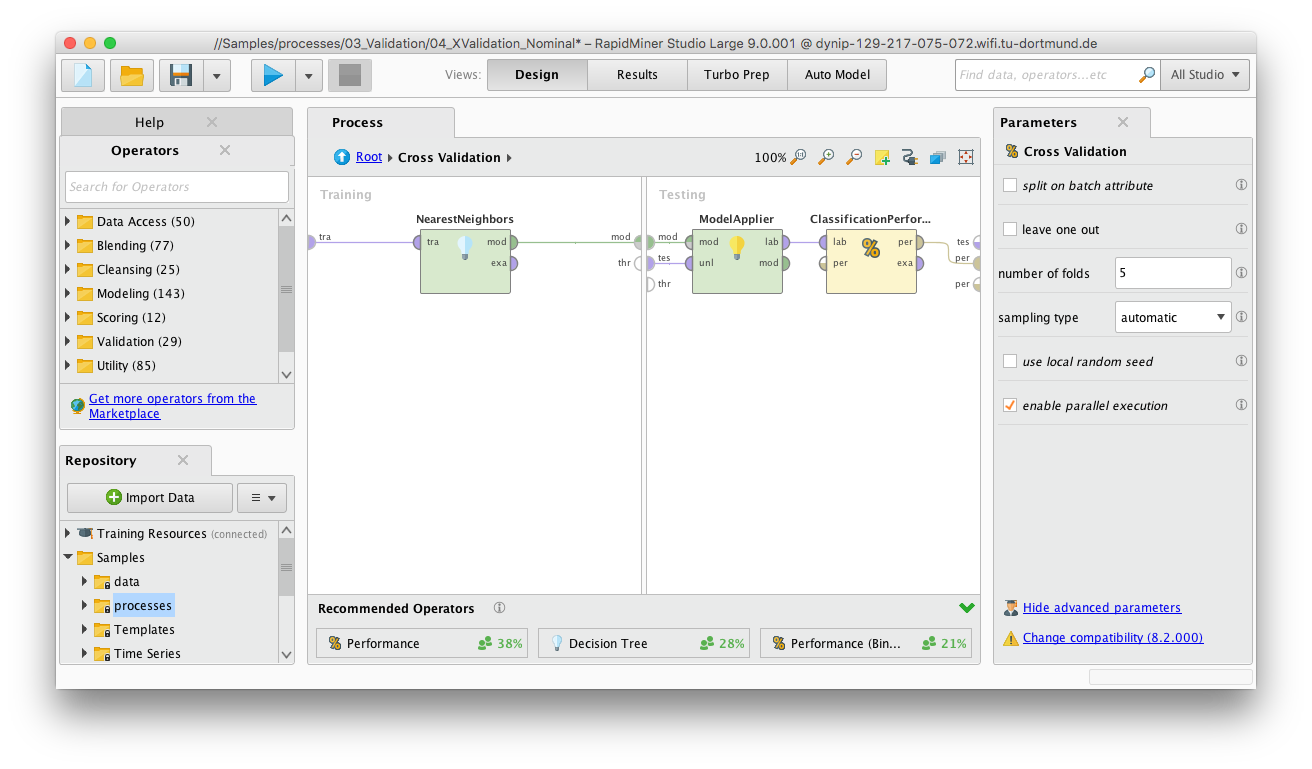
\includegraphics[width=\linewidth]{rapidminer.png}
\end{frame}

\begin{frame}[t,fragile]{Review}

    \begin{columns}[t]
    \begin{column}{0.5\textwidth}
    \begin{block}{Convenience}
        Has all the building blocks of routine machine learning tasks:
        \begin{itemize}
            \item Data Import, Filtering and Normalization
            \item Standard Machine Learning Methods
            \item Validation and Visualization
        \end{itemize}
        Implementing new methods is painful and under-documented.
    \end{block}
    \end{column}
    \begin{column}{0.5\textwidth}
    \begin{block}{Reproducibility}
        Let's write some stuff
        \begin{itemize}
        \item Exchangable XML specifications of data mining processes
        \item No Version Control of Process Files $\rightarrow$ Manual Versioning via FileNames
        \end{itemize}
    \end{block}
    
    \end{column}
    \end{columns}
    \hfill
    %\metroset{block=fill}
    %\begin{columns}\begin{column}{\textwidth}
    \begin{alertblock}{Takeaway Message}
        Rapidminer offers you the possibility to quickly evaluate the performance of a wide range of standard methods on a new data mining task.
    \end{alertblock}
    %\end{column}\end{columns}
\end{frame}

%Reihenfolge: Nach Büros, von Osten nach Westen und sekundär von Süden nach Norden
%Feel free to suggest changes
\section{Amal}
\begin{frame}[fragile]{EyeCatcher}
\end{frame}
\begin{frame}[t,fragile]{Review}
\end{frame}

\section{Katharina}
\begin{frame}[fragile]{EyeCatcher}
\end{frame}
\begin{frame}[t,fragile]{Review}
\end{frame}

\section{Alexey}
\begin{frame}[fragile]{EyeCatcher}
\end{frame}
\begin{frame}[t,fragile]{Review}
\end{frame}

\section{Mirko}
\begin{frame}[fragile]{Julia}
  \vspace*{2em}
  \hspace*{.025\textwidth} % center
  \begin{tikzpicture}
    \tikzstyle{textbox} = [
  below = 4mm,
  inner sep = 0pt,
  text centered
]

% dynamic vs static
\uncover<1->{%
  \draw[|-|, ultra thick] (0,0)
    node[textbox, text width=24mm] (dyn) {\Large Dynamic\\[-.1em]\footnotesize e.g. Python, R,\dots}
    -- (10,0)
    node[textbox, text width=26mm] (stat) {\Large Static\\[-.1em]\footnotesize e.g. C++, Java,\dots}
    node[midway, below=1mm] (jl) {};
}

% Julia
\uncover<2->{%
  \draw[<->, very thick, gray!66, dashed] ($(jl)+(-.8,-2mm)$) -- ($(jl)+(0,-1.2)$) -- ($(jl)+(+.8,-2mm)$);
  \draw[<-, very thick] (jl) -- +(0,-1.2) node[below=1mm] (jl-arrow) {};

  \node[
    anchor = north west,
    fill = lightgray!66,
    rounded corners,
    text width = 70mm,
    inner sep = 5mm,
    outer sep = 1mm
  ] (jl-box) at (jl-arrow -| dyn.west) {%
    \begin{columns}
    \begin{column}{.45\textwidth}
      \raggedleft
      
\includegraphics[width=.9\textwidth]{img/julia-logo}
    \end{column}
    \begin{column}{.55\textwidth}
      {\bfseries Flexibility + Speed:}
      \begin{itemize}
	\item JIT compilation
	\item optionally typed
	\item multiple dispatch
      \end{itemize}
    \end{column}
    \end{columns}
  };
}

% packages
\uncover<3->{%
  \node[
    below = 5mm,
    anchor = north east,
    text width = 25mm,
    align = right,
    inner sep = 1mm,
    xshift = -2mm,
    font = \bfseries
  ] (pkg) at (jl-arrow -| stat.east) {%
    DataFrames.jl\\
    PyCall.jl\\
    JuMP.jl\\
    Pkg.jl (in v1.0)\\
    \dots
  };

  \draw[thick, decoration={brace, mirror}, decorate] (pkg.north west) -- (pkg.south west)
    node[left=2.5mm, midway, anchor=east, font=\bfseries] {using};
}
  \end{tikzpicture}
\end{frame}
\begin{frame}[t,fragile]{Artifacts \scalebox{.85}{\enspace$\rightarrow$\enspace Reproducibility + Flexibility}}
  \vspace*{1.5em}
  \hspace*{-.075\textwidth} % center
  \begin{tikzpicture}
    \definecolor{yaml-bg}{HTML}{001B33}
\definecolor{yaml-prop}{HTML}{FF9D00}
\definecolor{yaml-str}{HTML}{3AD906}
\definecolor{yaml-num}{HTML}{FF0044}
\definecolor{tex-kw}{HTML}{F00000}
\definecolor{tex-env}{HTML}{5423D0}
\definecolor{tex-math}{HTML}{00A000}

% docker fill
\uncover<1->{%
  \fill[pattern=north east lines, pattern color=tu05light, rounded corners] (1.2,1.8) rectangle (6.6,-2.6)
    node[above left, anchor=south east, black!80] {\footnotesize Docker};
}

% meta-config
\uncover<2->{%
  \begin{scope}[scale=.78, transform shape, local bounding box=meta]
    \node[draw=gray, semithick, rectangle, fill=yaml-bg, text width=2cm, rounded corners, font=\ttfamily] at (0,0) {%
      \setlength{\baselineskip}{8pt}%
      \textcolor{yaml-prop}{\bfseries a\_1:} \textcolor{yaml-num}{1.0}\\[2pt]
      \textcolor{yaml-prop}{\bfseries dataset:}\\[1pt]
      \textcolor{white}{~~-} \textcolor{yaml-str}{fact}\\
      \textcolor{white}{~~-} \textcolor{yaml-str}{magic}
      \par % applies baselineskip to all lines
    };
  \end{scope}
  \node[below = 4mm, font=\small, align=center, text width=3cm] (metalab) at (meta.south) {Meta-Config\\[-2pt]\scriptsize(YAML)};
}

% job configs
\uncover<1->{%
  \begin{scope}[scale=.75, transform shape, shift={(3.25,-.1)}, local bounding box=jobs]
    \node[draw=gray, semithick, rectangle, fill=yaml-bg, text width=2.2cm, rounded corners, font=\ttfamily] at (.2,.2) {%
      \setlength{\baselineskip}{8pt}%
      \textcolor{yaml-prop}{\bfseries a\_1:} \textcolor{yaml-num}{1.0}\\[2pt]
      \textcolor{yaml-prop}{\bfseries data:} \textcolor{yaml-str}{magic}
      \par % applies baselineskip to all lines
    };
    \node[draw=gray, semithick, rectangle, fill=yaml-bg, text width=2.2cm, rounded corners, font=\ttfamily] at (0,0) {%
      \setlength{\baselineskip}{8pt}%
      \textcolor{yaml-prop}{\bfseries a\_1:} \textcolor{yaml-num}{1.0}\\[2pt]
      \textcolor{yaml-prop}{\bfseries data:} \textcolor{yaml-str}{fact}
      \par % applies baselineskip to all lines
    };
  \end{scope}
  \node[below, font=\small, align=center, text width=3cm] (joblab) at (jobs.south|-metalab.north) {Job Configs\\[-2pt]\scriptsize(YAML)};
}

% spectra
\uncover<1->{%
  \begin{scope}[scale=.85, transform shape, shift={(5.25,-.7)}, local bounding box=analysis]
    \begin{scope}[anchor=north east, shift={(.18,.18)}]
      % 
% This file was generated with Res.smearing_histogram("res/spectra/comparison_magic_uniform.csv"res/metrics/comparison_magic_uniform.csv")
% 
% git commit = c084a7e45bb1f3afd5999b1c80a6c3f4be207858
% git origin = git@bitbucket.org:mbunse/mt-exp.git
% uncommited changes = false
% 
\tikzstyle{every node} = [font=\small]

\begin{axis}[
  ylabel = {},
  xmin = {1.599999999999},
  xmax = {4.4000000000010004},
  xlabel = {},
  histogram axis,
  ymode = log,
  log origin y=infty,
  scale = .25,
  yticklabels = \empty,
  xticklabels = \empty,
  ylabel style = {rotate = 270, at = {(-.025,.5)}},
  xlabel style = {at = {(.5,-.025)}}
]
%   width = .75*\axisdefaultwidth,
%   height = .675*\axisdefaultheight,

% \addplot+[
%   histogram plot,
%   black,
%   thin,
%   name path = truth,
%   dash pattern={on 2.25pt off 0.75pt}
% ]
% coordinates {
%   (1.599999999999, 0.0)
%   (1.6, 0.06451926499999999)
%   (1.8333333333333333, 0.1221511)
%   (2.066666666666667, 0.1482697)
%   (2.3, 0.1439983)
%   (2.533333333333333, 0.1244045)
%   (2.7666666666666666, 0.10419795000000001)
%   (3.0, 0.08582171499999999)
%   (3.2333333333333334, 0.06412323500000001)
%   (3.466666666666667, 0.050539829999999994)
%   (3.7, 0.037032365)
%   (3.933333333333333, 0.027978120000000002)
%   (4.166666666666667, 0.026964024999999996)
%   (4.4, 0.026964024999999996)
%   (4.4000000000010004, 0.0)
% };
% \addlegendentry{$\mathbf{f}$}

\addplot+[
  histogram plot,
  tu02,
  very  thick,
  name path = estimate
]
coordinates {
  (1.599999999999, 0.0)
  (1.6, 0.07563379)
  (1.8333333333333333, 0.11441804999999998)
  (2.066666666666667, 0.14546300000000004)
  (2.3, 0.14178325)
  (2.533333333333333, 0.12264900000000004)
  (2.7666666666666666, 0.10740475000000001)
  (3.0, 0.086949075)
  (3.2333333333333334, 0.064010205)
  (3.466666666666667, 0.048701285000000004)
  (3.7, 0.03753382999999999)
  (3.933333333333333, 0.029620479999999998)
  (4.166666666666667, 0.025833409999999994)
  (4.4, 0.025833409999999994)
  (4.4000000000010004, 0.0)
};
% \addlegendentry{$\hat{\mathbf{f}}_\text{$\text{\sc Dsea}^+$}$}

% \addplot[draw=none, fill=tu01, fill opacity=0.33] fill between[of = truth and estimate];

% \legend{} % omit legend

\end{axis}


    \end{scope}
    \begin{scope}[anchor=north east, shift={(0,0)}]
      % 
% This file was generated with Res.smearing_histogram("res/spectra/comparison_magic_uniform.csv"res/metrics/comparison_magic_uniform.csv")
% 
% git commit = c084a7e45bb1f3afd5999b1c80a6c3f4be207858
% git origin = git@bitbucket.org:mbunse/mt-exp.git
% uncommited changes = false
% 
\tikzstyle{every node} = [font=\small]

\begin{axis}[
  ylabel = {$f$},
  xmin = {1.599999999999},
  xmax = {4.4000000000010004},
  xlabel = {energy},
  histogram axis,
  ymode = log,
  log origin y=infty,
  scale = .25,
  yticklabels = \empty,
  xticklabels = \empty,
  ylabel style = {rotate = 270, at = {(-.025,.5)}},
  xlabel style = {at = {(.5,-.025)}}
]
%   width = .75*\axisdefaultwidth,
%   height = .675*\axisdefaultheight,

% \addplot+[
%   histogram plot,
%   black,
%   thin,
%   name path = truth,
%   dash pattern={on 2.25pt off 0.75pt}
% ]
% coordinates {
%   (1.599999999999, 0.0)
%   (1.6, 0.06451926499999999)
%   (1.8333333333333333, 0.1221511)
%   (2.066666666666667, 0.1482697)
%   (2.3, 0.1439983)
%   (2.533333333333333, 0.1244045)
%   (2.7666666666666666, 0.10419795000000001)
%   (3.0, 0.08582171499999999)
%   (3.2333333333333334, 0.06412323500000001)
%   (3.466666666666667, 0.050539829999999994)
%   (3.7, 0.037032365)
%   (3.933333333333333, 0.027978120000000002)
%   (4.166666666666667, 0.026964024999999996)
%   (4.4, 0.026964024999999996)
%   (4.4000000000010004, 0.0)
% };
% \addlegendentry{$\mathbf{f}$}

\addplot+[
  histogram plot,
  tu01,
  very  thick,
  name path = estimate
]
coordinates {
  (1.599999999999, 0.0)
  (1.6, 0.07563379)
  (1.8333333333333333, 0.11441804999999998)
  (2.066666666666667, 0.14546300000000004)
  (2.3, 0.14178325)
  (2.533333333333333, 0.12264900000000004)
  (2.7666666666666666, 0.10740475000000001)
  (3.0, 0.086949075)
  (3.2333333333333334, 0.064010205)
  (3.466666666666667, 0.048701285000000004)
  (3.7, 0.03753382999999999)
  (3.933333333333333, 0.029620479999999998)
  (4.166666666666667, 0.025833409999999994)
  (4.4, 0.025833409999999994)
  (4.4000000000010004, 0.0)
};
% \addlegendentry{$\hat{\mathbf{f}}_\text{$\text{\sc Dsea}^+$}$}

% \addplot[draw=none, fill=tu01, fill opacity=0.33] fill between[of = truth and estimate];

% \legend{} % omit legend

\end{axis}


    \end{scope}
  \end{scope}
  \node[below, font=\small, align=center, text width=3cm] at (analysis.south|-metalab.north) {Analysis Results\\[-2pt]\scriptsize(CSV)};
}

% metrics
\uncover<3->{%
  \begin{scope}[scale=.75, transform shape, shift={(10.25,-.1)}, local bounding box=metrics]
    \node at (0,0) {%
      \scriptsize
      \setlength{\tabcolsep}{4pt}
      \renewcommand{\arraystretch}{1.12}
      \begin{tabular}{c|c|c}
	{\bf data} & {\bf k} & {\bf EMD} \\
	\hline
	fact & 1 & 0.12 \\[-2pt]
	fact & 2 & 0.08 \\[-2pt]
	magic & 1 & 0.14 \\[-2pt]
	\vdots & \vdots & \vdots
      \end{tabular}
    };
  \end{scope}
  \node[below, font=\small, align=center, text width=3cm] at (metrics.south|-metalab.north) {Metrics\\[-2pt]\scriptsize(CSV)};
}

% tex code
\uncover<5->{%
  \begin{scope}[scale=.8, transform shape, shift={(12.75,-.2)}, local bounding box=plot]
    \node[text width=2.4cm, font=\ttfamily, fill=lightgray!66, rounded corners, inner sep=6pt] at (0,0) {%
      \scriptsize
      \setlength{\baselineskip}{-0pt}%
      \textcolor{tex-kw}{\textbackslash begin}\{\textcolor{tex-env}{axis}\}[\\
      ~~ylabel = \{\textcolor{tex-math}{\$f\$}\},\\
      ~~xmin = \{1.59\},\\
      ~~xmax = \{4.40\},\\[3pt]
      ~~\dots
      \par
    };
  \end{scope}
  \node[below, font=\small, align=center, text width=3cm] (plotlab) at (plot.south|-metalab.north) {Plot\\[-2pt]\scriptsize(TeX)};
  \node[below=3mm, rotate=-9, font=\small\bfseries, align=center, text width=3cm, tu01] at (plotlab.south) {versioning info\\embedded!};
}

% plots / paper
\uncover<6->{%
  \begin{scope}[shift={(12.65,-.06)}, local bounding box=paper]
    \node[inner sep=0pt] at (0,0) {%
      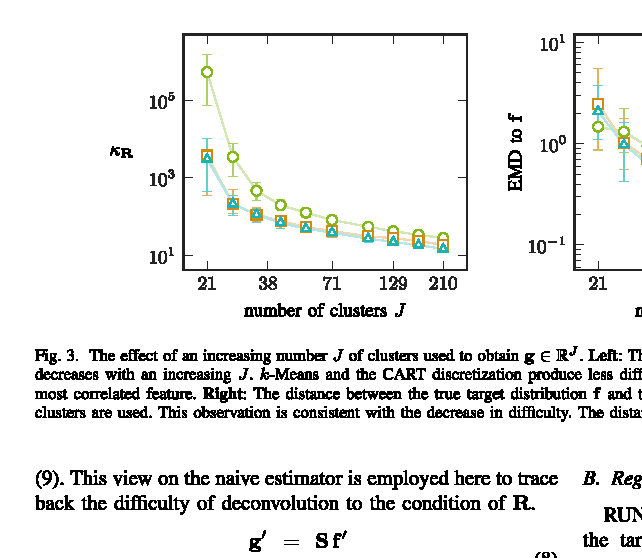
\includegraphics[scale=.16]{img/tex/embed}
    };
  \end{scope}
  \node[below, font=\small, align=center, text width=3cm] at (paper.south|-metalab.north) {Paper\\[-2pt]\scriptsize(PDF)};
}

% arrows
\uncover<2->{%
  \draw[thick] ($(meta.north)+(15pt,2pt)$) edge[->, bend left=50]
    node[pos=.45, above, font=\footnotesize] {split} ($(jobs.north)+(-15pt,2pt)$);
}
\uncover<1->{%
  \draw[thick] ($(jobs.north)+(15pt,2pt)$) edge[->, bend left=50]
    node[pos=.6, above, font=\footnotesize]  {run experiments} ($(analysis.north)+(-15pt,2pt)$);
}
\uncover<3->{%
  \draw[thick] ($(analysis.north)+(20pt,2pt)$) edge[->, bend left=50]
    node[pos=.5, above, font=\footnotesize]  {evaluate} ($(metrics.north)+(-10pt,2pt)$);
}
\uncover<5->{%
  \draw[thick] ($(metrics.north)+(15pt,2pt)$) edge[->, bend left=50]
    node[pos=.5, above, font=\footnotesize]  {aggregate} ($(plot.north)+(-20pt,2pt)$);
}
\uncover<6->{%
  \draw[thick] ($(plot.north)+(15pt,2pt)$) edge[->, bend left=50]
    node[pos=.5, above, font=\footnotesize]  {embed} ($(paper.north)+(-15pt,2pt)$);
}

% workflow
\uncover<4->{%
  \draw[<-, ultra thick] ($(jobs.south)+(0,-25mm)$) -- ($(jobs.south)+(0,-30mm)$)
    node[below=1mm, text width=4cm, align=center] (pushlab) {push code, data \& configs};
  \draw[->, ultra thick] ($(jobs.south)+(2.75,-25mm)$) -- ($(jobs.south)+(2.75,-30mm)$)
    node[below=1mm, text width=4cm, align=center] {pull\\results};
}
  \end{tikzpicture}
\end{frame}

\section{Sebastian}
\begin{frame}[fragile]{\textbf{Goal:} Machine Learning on Embedded Systems $\to$ \texttt{C/C++} is de-facto standard}
    \pause
    \begin{columns}
        \begin{column}{0.6\textwidth}
            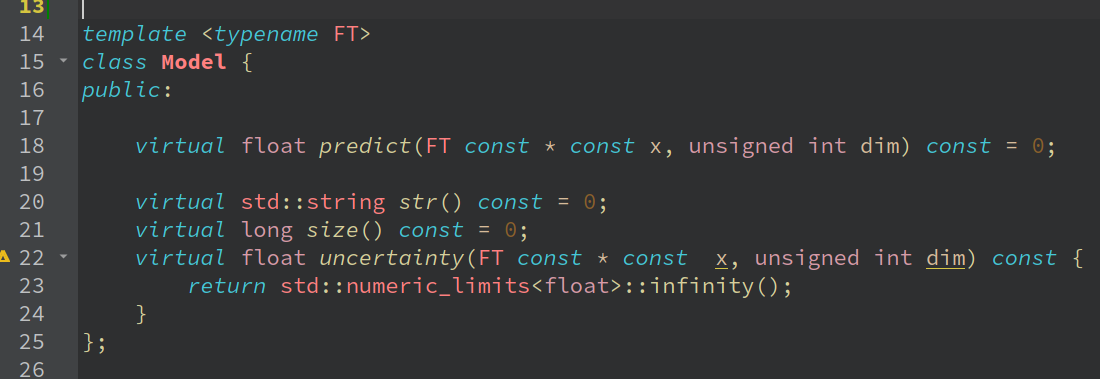
\includegraphics[width=\textwidth]{img/sebastian-cpp.png}
        \end{column}
        
        \begin{column}{0.4\textwidth}
            \vspace{0.2cm}

            PROs
            \begin{itemize}
                \item Fast \& Small memory footprint
                \item We know what we are doing
                \item `Old'/Well-known tool-chain
            \end{itemize}
            CONs
            \begin{itemize}
                \item Sometimes tedious work
                \item Somewhat difficult to debug
            \end{itemize}
        \end{column}
    \end{columns}

    \pause
    \vspace{-0.2cm}
    \textbf{Thus} Keep speed, but make tedious work less tedious
    \pause 

    \begin{itemize}
         \item \texttt{QTCreator} In-built debugger / project management \pause
         %\item \texttt{CMake/Make} Build-System for dependency management
         \item \texttt{STL} For convenience function (e.g. \texttt{std::map}, \texttt{std::vector} etc.) \pause
         \item \texttt{OpenBlas/MKL} For (fast) math functions (e.g. \texttt{LAPACKE\_spotri}) \pause
         \item \texttt{OpenMP} For parallelization (e.g. \texttt{\#pragma omp parallel}) \pause
         \item \texttt{Python (etal.)} Data pre-processing ($\to$ export data as CSV)
     \end{itemize} 
\end{frame}

\begin{frame}[t,fragile]{Excursus: FPGA Development}
    \hspace{-0.4cm}\textbf{General Workflow}

    \begin{center}
        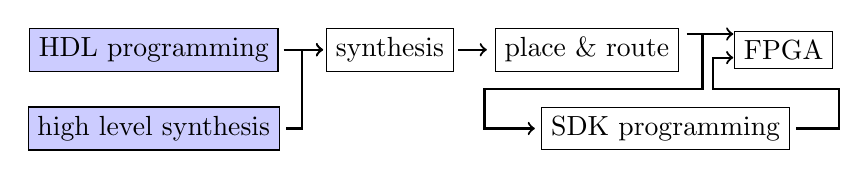
\begin{tikzpicture}
            \node[rectangle,draw, fill=blue!20] at (0,0) {high level synthesis};
            \node[rectangle,draw, fill=blue!20] at (0,1) {HDL programming};
            \node[rectangle,draw] at (3,1) {synthesis};
            \node[rectangle,draw] at (5.5,1) {place \& route};
            \node[rectangle,draw] at (6.5,0) {SDK programming};
            \node[rectangle,draw] at (8.0,1) {FPGA};
            %smooth, tension=0.05
            %\draw plot [->,thick]  coordinates {(1.68,0) (1.88, 0.) (1.88,1) (2.15,1)};
            \draw[->,thick] (1.68,0) -- (1.88, 0) -- (1.88,1) -- (2.15,1);
            \draw[->,thick] (1.65,1) -- (2.15,1);
            \draw[->,thick] (3.87,1) -- (4.23,1);
            \draw[->, thick] (6.77,1.2) -- (6.97,1.2) -- (6.97, 0.5) -- (4.2,0.5) -- (4.2, 0) -- (4.84, 0);
            \draw[->, thick] (8.16,0) -- (8.7,0) -- (8.7, 0.5) -- (7.1,0.5) -- (7.1, 0.9) -- (7.36,0.9);
            \draw[->,thick] (6.77,1.2) -- (7.36,1.2);
        \end{tikzpicture}
    \end{center}

    \pause
    \begin{columns}
        \begin{column}{0.5\textwidth}
            \textbf{Hardware Description Language (HDL)}
            \begin{itemize}
                \item Bit-Level/Register-Transfer-Level
                \item Usually simulated before put on an FPGA
                \item Slow / Tedious to develop, but ultimate control over hardware
                \item \textbf{Xilinx FPGAs} \texttt{Vivado}
            \end{itemize}
        \end{column}
        
        \begin{column}{0.5\textwidth}
            \textbf{High Level Synthesis (HLS)}
            \begin{itemize}
                \item Compile \texttt{C/C++/OpenCL} $\to$ HDL
                \item Usually tested on CPU, then put on FPGA
                \item Faster to develop with, but less control over hardware
                \item \textbf{Xilinx FPGAs} \texttt{Vivado HLS} or \texttt{SDSoC}
            \end{itemize}
        \end{column}
    \end{columns}
\end{frame}

\begin{frame}[t,fragile]{Excursus: FPGA Development}
    \hspace{-0.4cm}\textbf{General Workflow}

    \begin{center}
        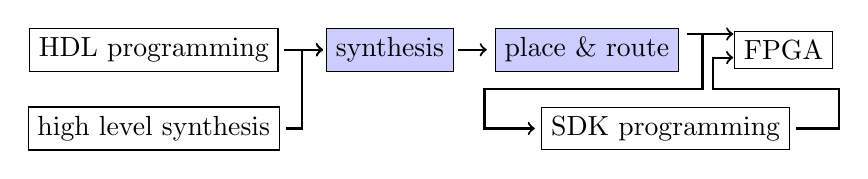
\begin{tikzpicture}
            \node[rectangle,draw] at (0,0) {high level synthesis};
            \node[rectangle,draw] at (0,1) {HDL programming};
            \node[rectangle,draw, fill=blue!20] at (3,1) {synthesis};
            \node[rectangle,draw, fill=blue!20] at (5.5,1) {place \& route};
            \node[rectangle,draw] at (6.5,0) {SDK programming};
            \node[rectangle,draw] at (8.0,1) {FPGA};
            %smooth, tension=0.05
            %\draw plot [->,thick]  coordinates {(1.68,0) (1.88, 0.) (1.88,1) (2.15,1)};
            \draw[->,thick] (1.68,0) -- (1.88, 0) -- (1.88,1) -- (2.15,1);
            \draw[->,thick] (1.65,1) -- (2.15,1);
            \draw[->,thick] (3.87,1) -- (4.23,1);
            \draw[->, thick] (6.77,1.2) -- (6.97,1.2) -- (6.97, 0.5) -- (4.2,0.5) -- (4.2, 0) -- (4.84, 0);
            \draw[->, thick] (8.16,0) -- (8.7,0) -- (8.7, 0.5) -- (7.1,0.5) -- (7.1, 0.9) -- (7.36,0.9);
            \draw[->,thick] (6.77,1.2) -- (7.36,1.2);
        \end{tikzpicture}
    \end{center}

    \pause
    \textbf{Synthesis} Calculate specific FPGA configurations 
    
    \textbf{Place \& Route} Calculate signal routing 
    
    \pause
    \textbf{Xilinx FPGAs} Vivado \texttt{or} SDSoC
    \begin{itemize}
        \item Takes a long time $\to$ store as many checkpoints as possible
        \item Start with small configurations, e.g. clock hat $100$Mhz
        \item Start with less aggressive optimizations
    \end{itemize}
    $\Rightarrow$ HW Description (XML-File), Block RAM Memory Map (BMM-File), FPGA Bitsream 
\end{frame} 

\begin{frame}[t,fragile]{Excursus: FPGA Development}
    \hspace{-0.4cm}\textbf{General Workflow}
    \begin{center}
        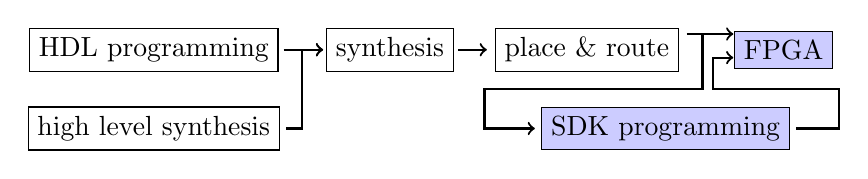
\begin{tikzpicture}
            \node[rectangle,draw] at (0,0) {high level synthesis};
            \node[rectangle,draw] at (0,1) {HDL programming};
            \node[rectangle,draw] at (3,1) {synthesis};
            \node[rectangle,draw] at (5.5,1) {place \& route};
            \node[rectangle,draw,fill=blue!20] at (6.5,0) {SDK programming};
            \node[rectangle,draw, fill=blue!20] at (8.0,1) {FPGA};
            %smooth, tension=0.05
            %\draw plot [->,thick]  coordinates {(1.68,0) (1.88, 0.) (1.88,1) (2.15,1)};
            \draw[->,thick] (1.68,0) -- (1.88, 0) -- (1.88,1) -- (2.15,1);
            \draw[->,thick] (1.65,1) -- (2.15,1);
            \draw[->,thick] (3.87,1) -- (4.23,1);
            \draw[->, thick] (6.77,1.2) -- (6.97,1.2) -- (6.97, 0.5) -- (4.2,0.5) -- (4.2, 0) -- (4.84, 0);
            \draw[->, thick] (8.16,0) -- (8.7,0) -- (8.7, 0.5) -- (7.1,0.5) -- (7.1, 0.9) -- (7.36,0.9);
            \draw[->,thick] (6.77,1.2) -- (7.36,1.2);
        \end{tikzpicture}
    \end{center}

    \pause
    \textbf{SDK programming} If HW Description contains programmable devices (e.g. CPU)
    \begin{itemize}
        \item Load HW Description File and BMM file
        \item Configure Board Support Package (e.g. Filesystem, Ethernet...)
        \item Implement functionality in \texttt{C/C++}
    \end{itemize}
    
    \pause
    \textbf{Then} Flash Bitstream using \texttt{Vivado} \& flash microcode using \texttt{Vivado SDK} 

    \textbf{Note} For some devices families (e.g. Zynq), \texttt{SDSoC} encapsulates all steps in one tool
\end{frame}

\section{Lukas}
\begin{frame}[t,fragile]{Python: Sacred Experiments and Git Versioning}
\vspace{-1.45mm}
\begin{columns}
\begin{column}{.45\paperwidth}
    % \includegraphics[keepaspectratio,width=\paperwidth]{trello}    
    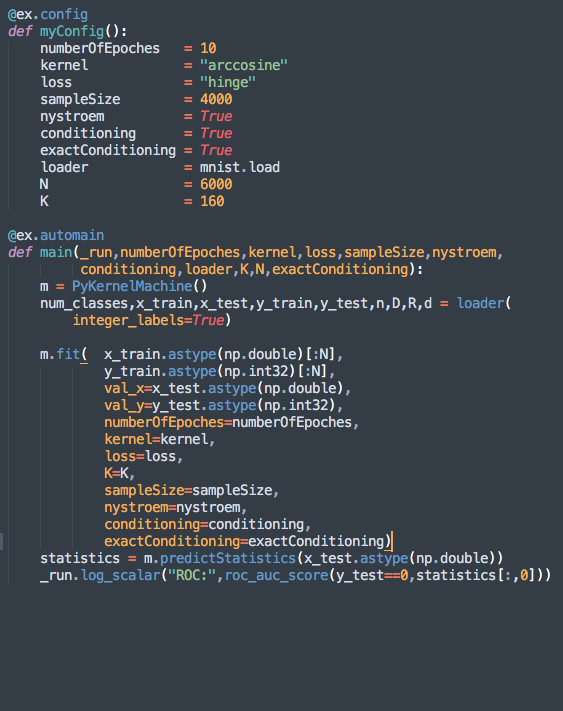
\includegraphics[width=\textwidth]{sacred}
\end{column}
\begin{column}{.05\paperwidth}
    
\end{column}
\begin{column}{.5\paperwidth}
    What is an \alert{experiment}?
    \begin{itemize}
        \item Python-Script + Libraries (standard + own c++)
        \item Parameters
        \item Results (Standard-Output, Metrics, \emph{Files})
    \end{itemize}
    Sacred logs
    \begin{itemize}
        \item git status (commit-hash + patch)
        \item python status (version, maybe libaries?)
        \item standard output (+ regex-metrics)
        \item metrics via logging functions
    \end{itemize}
    in a database. 

    There are various \alert{front-ends} to this database.
    \vspace{1cm}
\end{column}
\end{columns}
\end{frame}

\begin{frame}[t,fragile]{Review}
\end{frame}
\begin{frame}[fragile]{Resources}
\begin{tabular}{ll}
    Sacred:&\url{https://github.com/IDSIA/sacred}\\
    Omni-Board:& \url{https://github.com/vivekratnavel/omniboard}\\
\end{tabular}
\end{frame}

\section{Sibylle}
\begin{frame}[fragile]{Julia + Jupyter Notebook}
\begin{columns}
\begin{column}{0.7\textwidth}
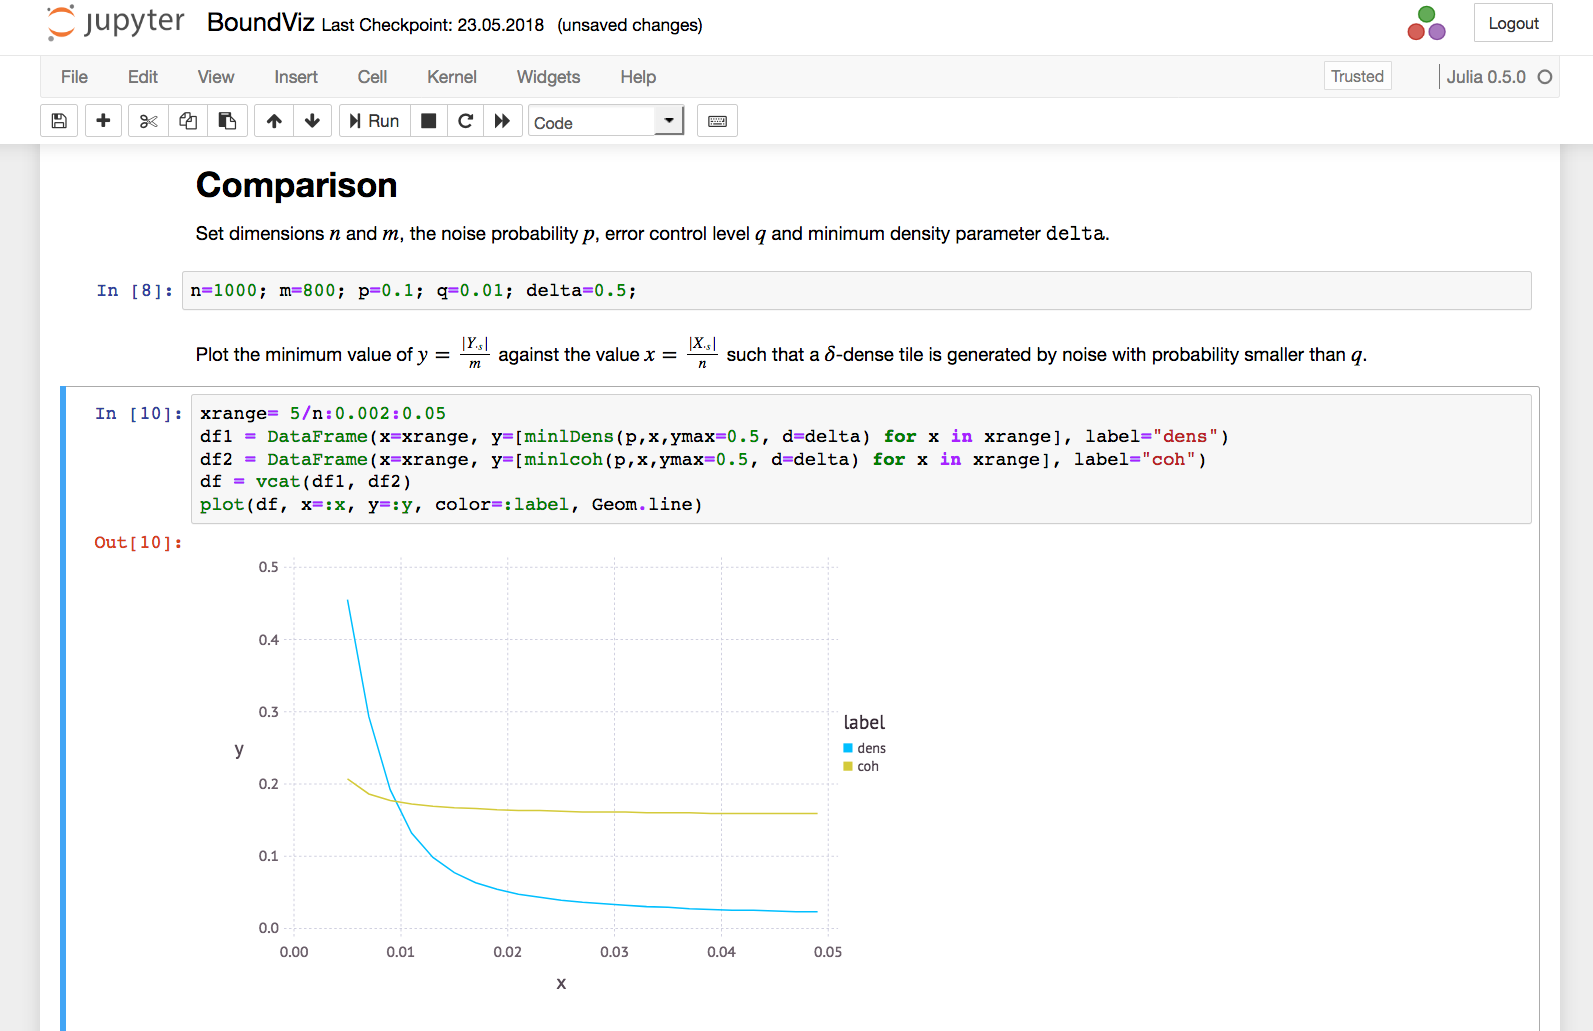
\includegraphics[width=\textwidth]{julia.png}
\end{column}
\begin{column}{0.25\textwidth}
PROs
\begin{itemize}
    \item Readability
    \item No installation necessary
    \item Python integration
\end{itemize}
CONs
\begin{itemize}
    \item Syntax changes with each version
    \item Performance issues
\end{itemize}
\end{column}
\end{columns}
\end{frame}

\begin{frame}[t,fragile]{Workflow}
\begin{enumerate}
    \item Data preprocessing, generation of synthetic experiments: IJulia script
    \item Algorithm implementation: Cublas C++, Python
    \item Experiment evaluation: IJulia script
\end{enumerate}
\end{frame}

\section{Thomas}
\begin{frame}[fragile]{EyeCatcher}
\end{frame}
\begin{frame}[t,fragile]{Review}
\end{frame}


\section{Discussion}
\begin{frame}[standout]{Discussion}
\begin{center}
    \LARGE{Although I assume it is already way past noon, maybe we still want to discuss some more?}
\end{center}
\end{frame}




\end{document}